\section{Результаты работы третьей лабораторной работы}


\subsection{Назанчение ресурсов задачам}

\begin{figure}[ht!]
	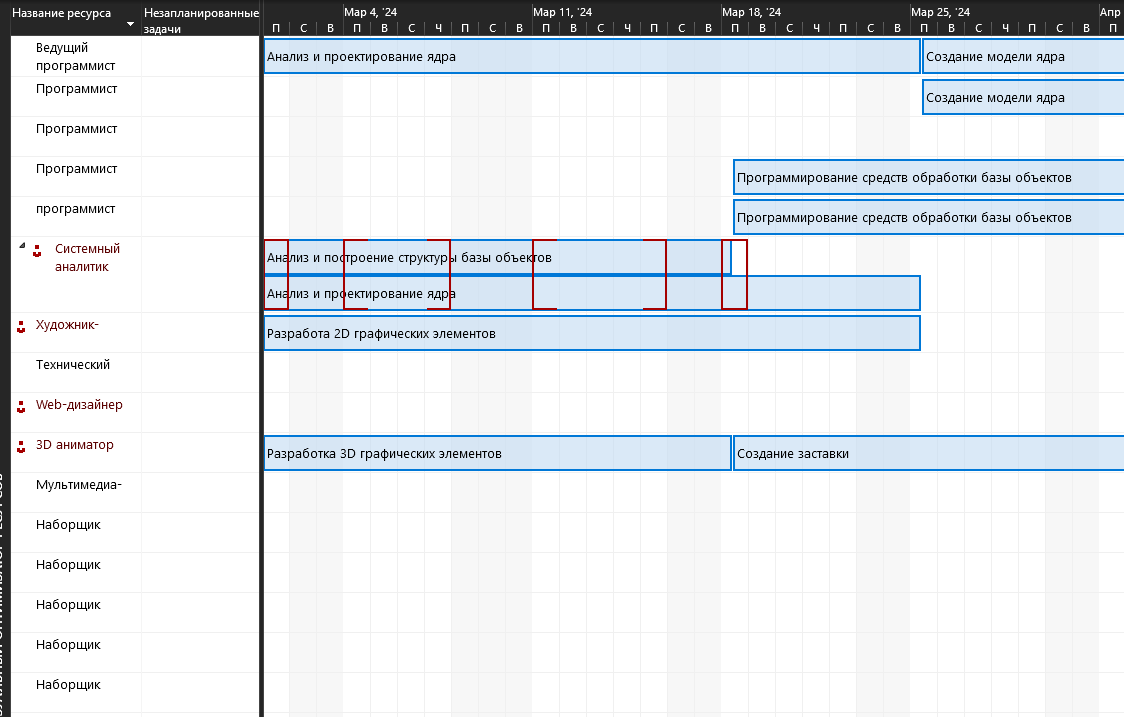
\includegraphics[width=0.75\linewidth]{assets/images/conflicts.png}
	\label{fig:r2}
	\caption{Ресусры}
\end{figure}
\FloatBarrier

Видно, что у художника-дизайнера задачи (разработка дизайна руководства и разработка дизайна сайта) накладываются друг на друга и он не успевает их выполнить.
У технического писателя --- написание руководства пользователя и создание справочной системы.
У системного аналитика --- анализ и построение структуры объектов, и анализ и проектирование ядра.

\begin{figure}[ht!]
	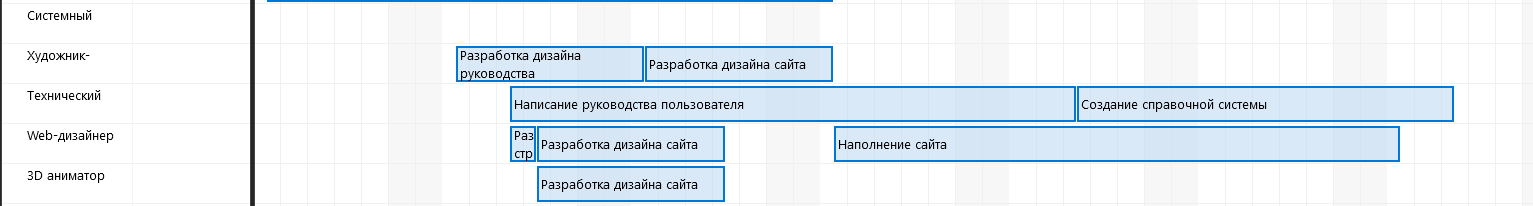
\includegraphics[width=0.75\linewidth]{assets/images/conflicts-optimize.png}
	\label{fig:r2}
	\caption{Ресусры}
\end{figure}
\FloatBarrier

Таким образом, «Создание справочной системы» теперь должно выполняться не параллельно с задачей «Написание руководства пользователя», а сразу после неё. Произошло это из-за того, что «Написание руководства пользователя» находится на критическом пути.
Аналогично с задачей «Разработка сайта».

Сроки сдвинулись на 23 число.

\subsubsection{Задание 2}

Было создано повторяющееся событие --- «Совещание». 

\begin{figure}[ht!]
	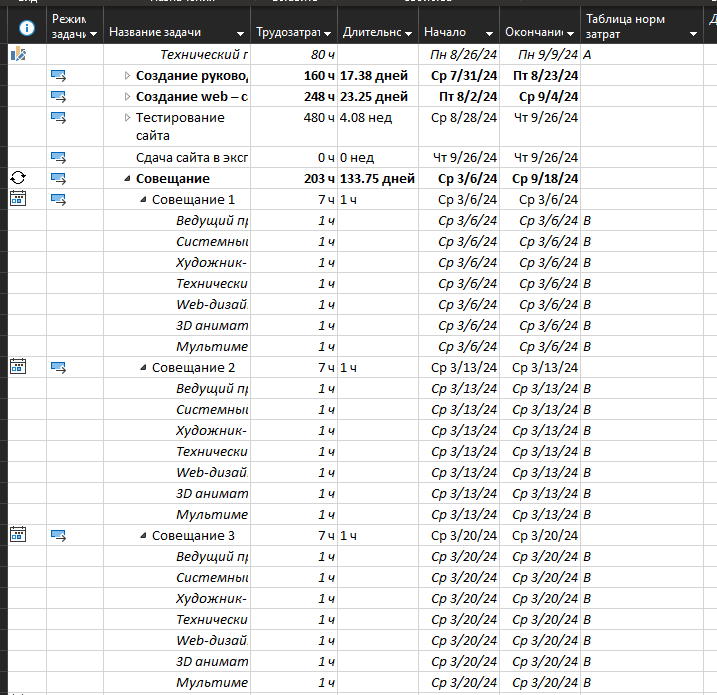
\includegraphics[width=0.75\linewidth]{assets/images/sovesh.png}
	\label{fig:r2}
	\caption{Совещание}
\end{figure}
\FloatBarrier

Назначены участники и устранена перегрузка ресурсов.
Возникли перегрузки из-за того, что совещания происходят в рабочее время, необходимо провести устранение перегрузки.

Для выравнивания было использовано автоматическое выравнивание. Т.к. перегружено сразу несколько ресурсов.

Таким образом, были добавлены перерывы в выполнении задач для совещаний, поэтому срок увеличился до 26.09.2022, поэтому увеличились и денежные затраты: 68 171.00 рублей, что превышает выделенный бюджет.

\begin{figure}[ht!]
	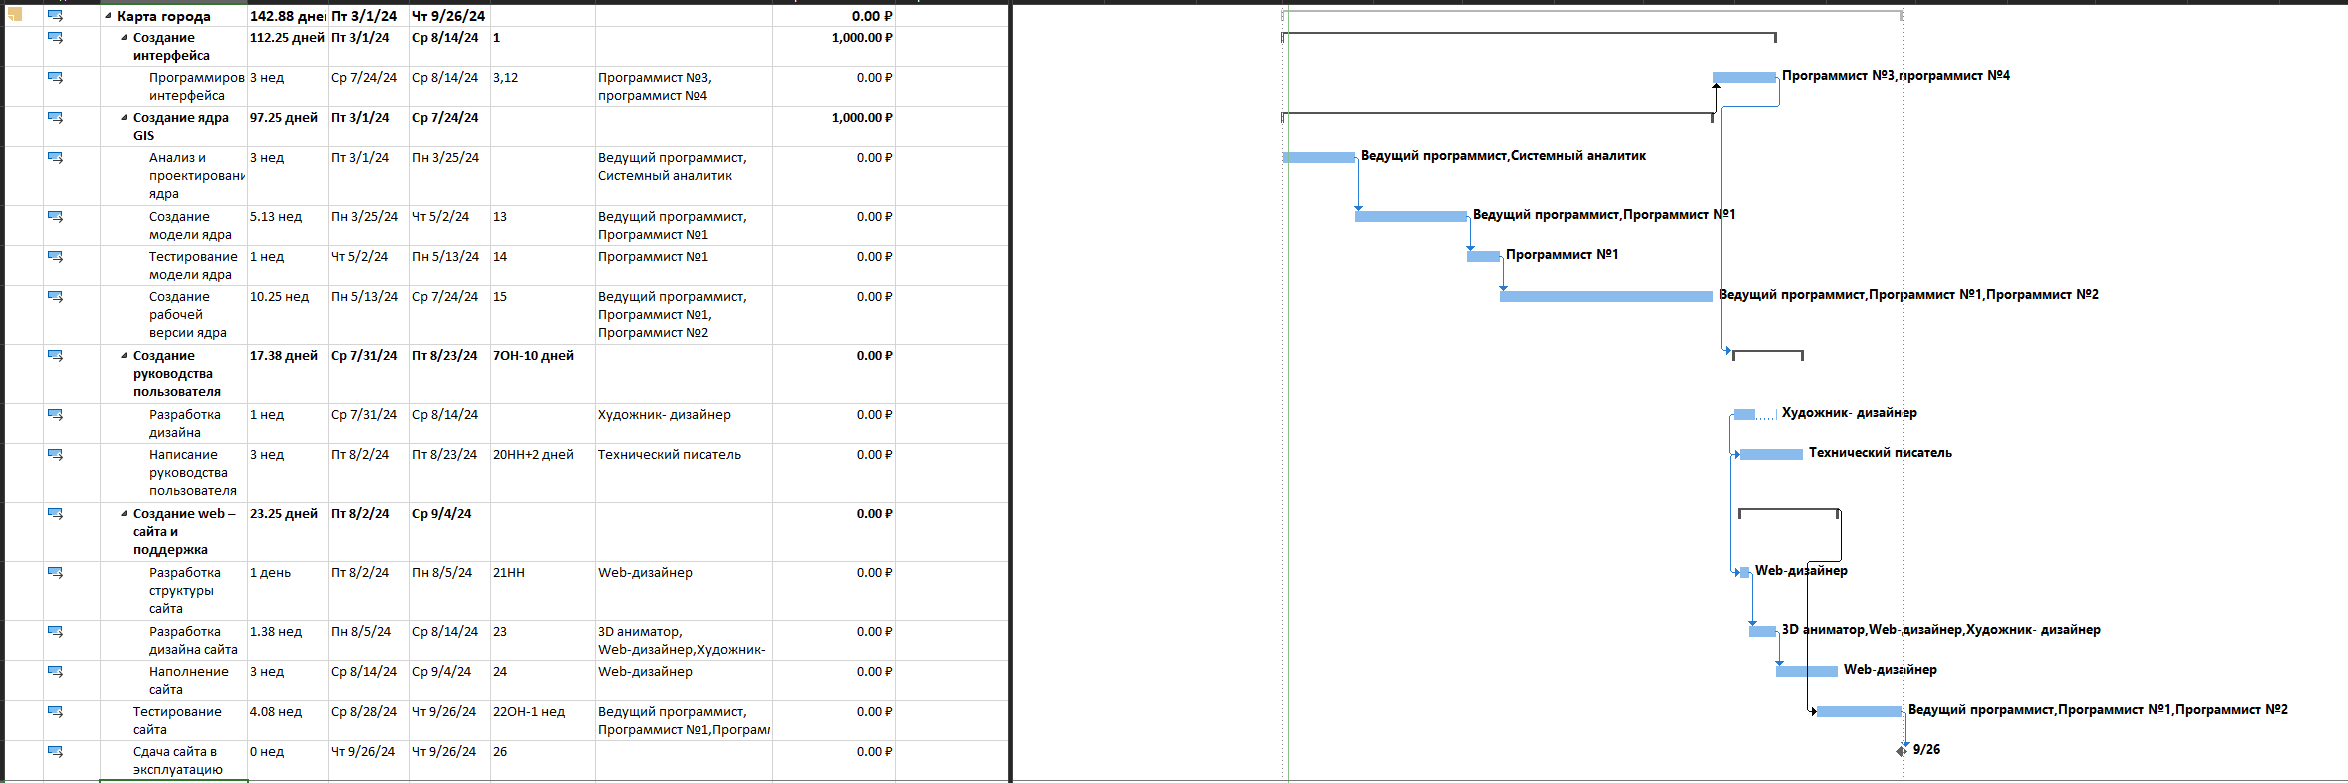
\includegraphics[width=0.75\linewidth]{assets/images/gant-new.png}
	\label{fig:r2}
	\caption{Новые сроки}
\end{figure}
\FloatBarrier

\begin{figure}[ht!]
	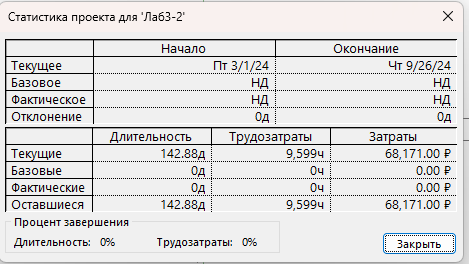
\includegraphics[width=0.75\linewidth]{assets/images/stat-1.png}
	\label{fig:r2}
	\caption{Новый бюджет}
\end{figure}
\FloatBarrier


Поскольку превышены и сроки, и затраты необходимо провести оптимизацию проекта. Поскольку на время совещания сотрудники не заняты своей основной работой, то необходимо пересмотреть план оплаты.

\begin{figure}[ht!]
	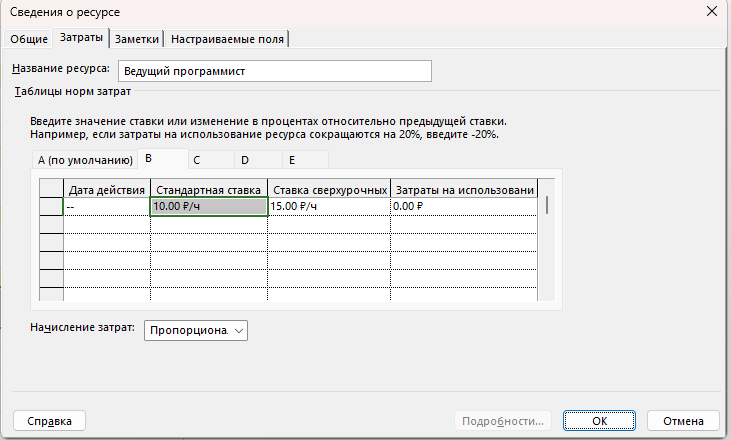
\includegraphics[width=0.75\linewidth]{assets/images/optimaz-1.png}
	\label{fig:r2}
	\caption{Не платим за совещаниея}
\end{figure}
\FloatBarrier

Внесём изменение в столбец «Таблица затрат»:

\begin{figure}[ht!]
	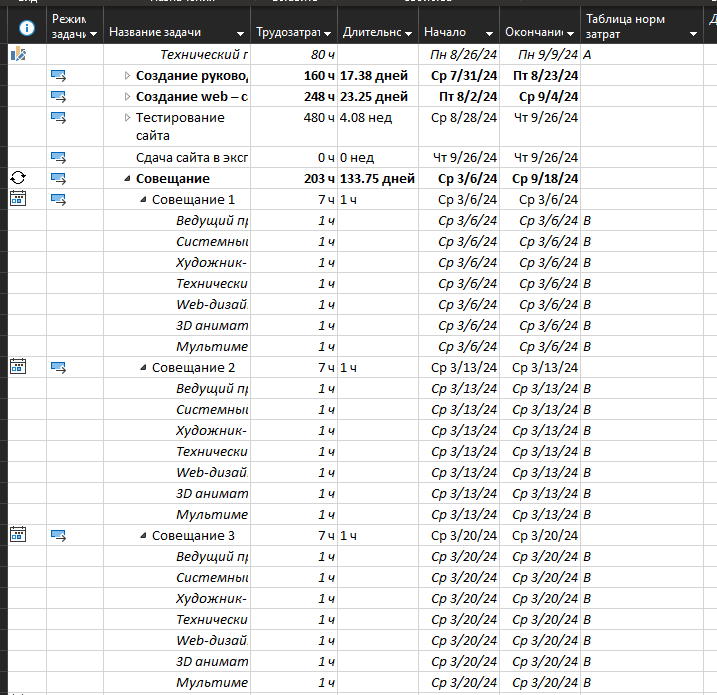
\includegraphics[width=0.75\linewidth]{assets/images/sovesh.png}
	\label{fig:r2}
	\caption{Не платим за совещаниея}
\end{figure}
\FloatBarrier

Таким образом, затраты уменьшились, и теперь находятся в рамках выделенного бюджета:

\begin{figure}[ht!]
	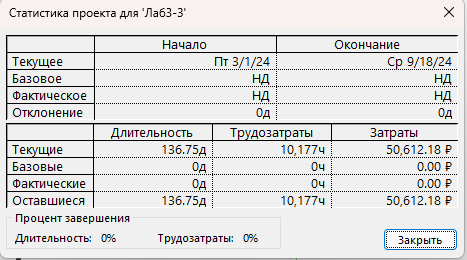
\includegraphics[width=0.75\linewidth]{assets/images/optimize-money.png}
	\label{fig:r2}
	\caption{Не платим за совещаниея}
\end{figure}
\FloatBarrier

\subsubsection{Задание 3}

Во вкладке Вид -> Фильтр –> Критические задачи отобразим Критические задачи проекта:


\begin{figure}[ht!]
	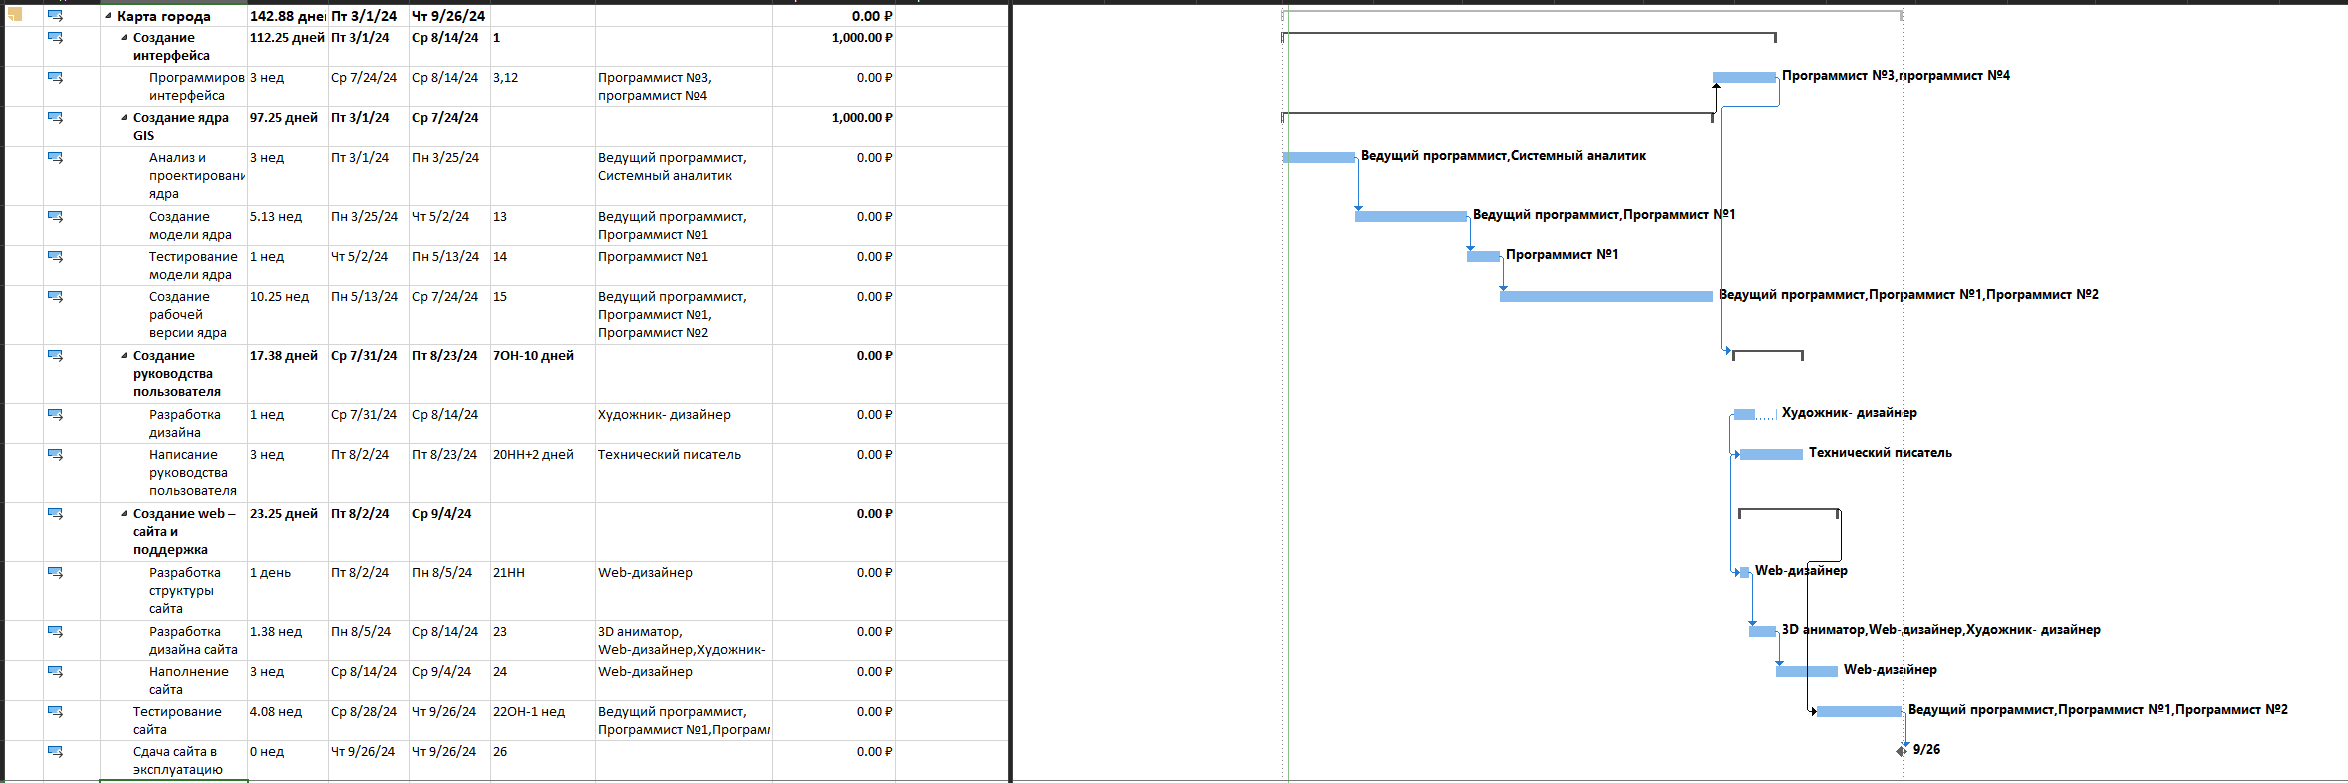
\includegraphics[width=0.75\linewidth]{assets/images/gant-new.png}
	\label{fig:r2}
	\caption{Критические задачи проекта}
\end{figure}
\FloatBarrier

Чтобы уменьшить длительность проекта, добавим других программистов туда, где работает только несколько.

\begin{figure}[ht!]
	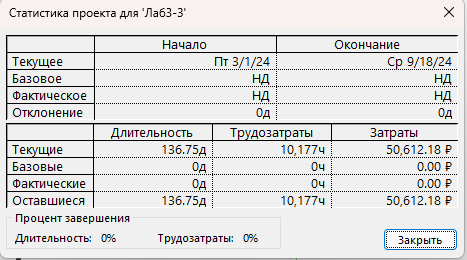
\includegraphics[width=0.75\linewidth]{assets/images/optimize-money.png}
	\label{fig:r2}
	\caption{Больше программистов}
\end{figure}
\FloatBarrier

Рассмотрим соотношение:

\begin{figure}[ht!]
	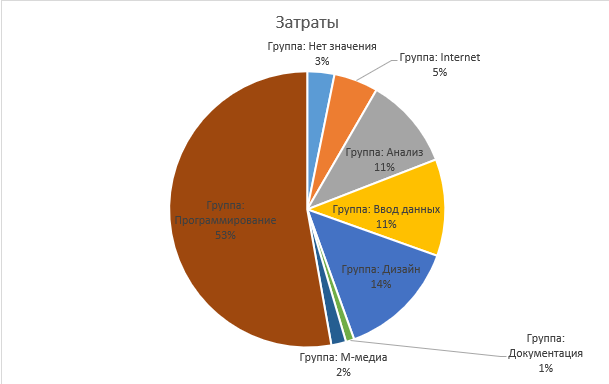
\includegraphics[width=0.75\linewidth]{assets/images/zatrat-2.png}
	\label{fig:r2}
	\caption{Прошлые}
\end{figure}
\FloatBarrier

\begin{figure}[ht!]
	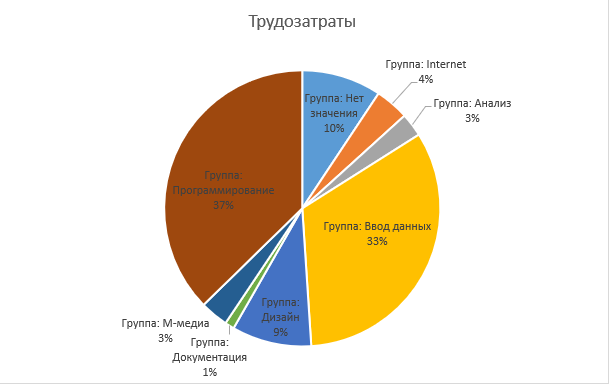
\includegraphics[width=0.75\linewidth]{assets/images/tryd-2.png}
	\label{fig:r2}
	\caption{Прошлые}
\end{figure}
\FloatBarrier

\begin{figure}[ht!]
	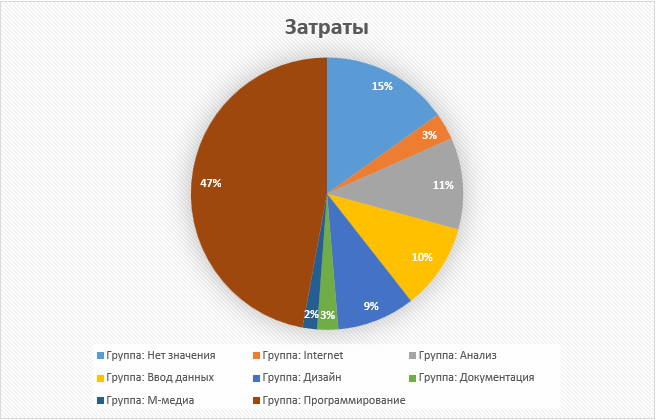
\includegraphics[width=0.75\linewidth]{assets/images/zatrat-3.png}
	\label{fig:r2}
	\caption{Новые}
\end{figure}
\FloatBarrier

\begin{figure}[ht!]
	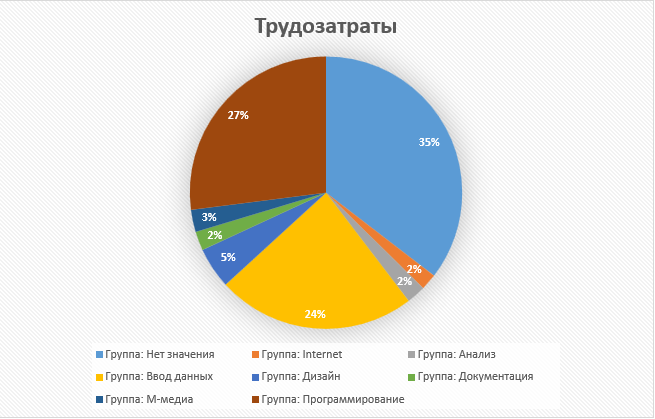
\includegraphics[width=0.75\linewidth]{assets/images/tryd-3.png}
	\label{fig:r2}
	\caption{Новые}
\end{figure}
\FloatBarrier

Таким образом, соотношение трудозатрат к затратам практически не изменилось. Увеличились затраты на программистов (около 3%).

За счет фиксированных трудовых рессурсов, при назначании программистов на задачи, было сокращено время задач.

\subsection*{Вывод}

В результате лабораторной работы были отработаны навыки использования программы Microsoft Project для оптимизации временных и финансовых показателей проекта. Для оптимизации затрат было решено создать второй план оплаты для сотрудников, участвующих в совещаниях, также для сокращения сроков было предпринято перераспределение работников (добавление программистов к задачам, где привлекаются лишь некоторые из них). 
Итак, затраты составляют 49 109,71 руб. (было 48 076,67), что находится в рамках выделенного бюджета, дата окончания проекта –-- 18.09.2022 (была 19.09.2022).
